%-*-coding: utf-8-*-
\FloatBarrier
\chapter{Описание используемого подхода}

\FloatBarrier
\section{Основная идея}

Идея заключается в составлении булевой формулы для набора входных деревьев и гибридизационного числа $h$, которая выполнима тогда и только тогда, когда существует гибридизационная сеть $N_h$ с гибридизационным числом $h$, содержащая в себе все входные деревья.
Определив диапазон возможных значений гибридизационного числа, можно перебрать их все и составить формулы для фиксированных значений гибридизационного числа.
В итоге, ответом на задачу будет та из выполнимых формул, которая соответствует наименьшему гибридизационному числу.

\FloatBarrier
\section{Препроцессинг}

Перед тем как приступать к непосредственному кодированию булевой формулы, применяются несколько эвристик, позволяющих разбить задачу на подзадачи, и следовательно уменьшить её сложность.
Для разбиения применяются следующие правила~\cite{bonet2009efficiently}:

\begin{enumerate}
	\item \textbf{Сокращение поддерева.} Если существует поддерево, содержащееся в каждом из исходных деревьев, значит в этой части эволюционной истории не наблюдалось ретикуляций, и для её отображения достаточно древовидной структуры.
	Поэтому во всех исходных деревьях следует заменить это поддерево на лист с новой меткой.
	После решения задачи, в готовой сети, следует заменить этот лист на исходное поддерево.
	\item \textbf{Сокращение кластера.} Если существует кластер $A$, содержащийся в каждом из исходных деревьев, его также следует заменить на лист с новой меткой, а задачу построения минимальной гибридизационной сети решать для этого кластера отдельно.
	После решения задачи, следует заменить этот лист в готовой сети на сеть, являющуюся решением задачи для кластера $A$.
\end{enumerate}

Предложенный далее алгоритм предполагает, что у всех входных деревьев общий корень, но это предположение не выполняется для построенных подзадач.
Поэтому следует добавить фиктивный корень ко всем деревьям в каждой из подзадач.
Чтобы сохранить структуру деревьев корень добавляется вместе с новым фиктивным листом.
Этот процесс проиллюстрирован на Рис.~\ref{dummy-example}.
После решения задачи, фиктивный корень и фиктивный лист следует удалить.

\begin{figure}[t]
  \centering{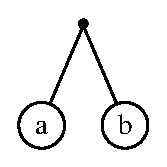
\includegraphics[width=2.6cm]{img/inp_dummy.eps}}
  \hspace{2cm}
  \centering{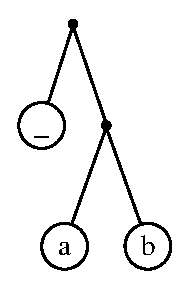
\includegraphics[width=3cm]{img/ans_dummy.eps}}
  \caption{Добавление фиктивного корня к дереву.}
  \label{dummy-example}
\end{figure}

\FloatBarrier
\section{Перебор гибридизационного числа}

Для решения задачи требуется найти такое минимальное $h$, что будет существовать гибридизационная сеть с гибридизационным числом равным $h$.
Существует несколько методик перебора значения $h$: последовательный перебор от больших значений к маленьким, от маленьких значений к большим и двоичный поиск.
В рамках данной работы были реализованы все три методики.
Если минимальное гибридизационное число равно $h_\mathrm{min}$, то, как правило, наибольшее количество вычислений потребуется для решения формулы при $h = h_\mathrm{min} - 1$.
Это обусловлено тем фактом, что найти какое-нибудь решение для солвера проще, чем, перебрав все варианты, убедиться, что решения не существует.
Экспериментальные результаты подтверждают это наблюдение, и поэтому перебор от маленьких значений к большим не представляет интереса, так как его производительность значительно ниже чем у остальных методов.
Результаты двоичного поиска практически повторяют результаты перебора от больших значений к маленьким, кроме случаев, в которых выполняется значительное количество проверок для значений меньших чем $h_\mathrm{min}$.


В данной работе используется перебор от больших значений к маленьким, как наиболее производительный метод.
Кроме того, было экспериментально обнаружено, что у многих из получаемых подзадач гибридизационное число мало, и времени на решение таких подзадач тратится мало, поэтому используется следующая эвристика: перед началом перебора производится попытка быстрого решения со значениями $h$ равными $0$, $1$, $2$ и $3$. В каждом из случаев солверу выделяется одна секунда на решение.


Объем вычислений можно очевидным образом сократить, если подобрать более точные границы возможных значений гибридизационного числа.
Существует несколько быстрых методов, основанных на различных эвристиках и методах линейного программирования, например PIRN$\mathrm{_{CH}}$~\cite{wu2010close}, RIATA-HGT~\cite{nakhleh2005riata} и MURPAR~\cite{park2012murpar}.

\FloatBarrier
\section{Кодирование булевой формулы}

\subsection{Общие замечания}

Обозначим исходное множество деревьев за $T$, множество таксонов за $A$, размер $A$ за $n$, а предполагаемое гибридизационное число за $h$. Требуется построить булеву формулу, которая выполнима тогда и только тогда, когда существует сеть, с гибридизационным номером $h$, в которой содержатся все деревья из $T$.

Для начала, заметим, что исходные деревья содержат $2 n - 1$ вершин, а искомая сеть состоит из $2 (n + k) + 1$ вершин, т.к. добавляется фиктивный корень и фиктивный лист. Среди этих вершин $n + 1$ лист, $k$ ретикулярных вершин, и $n + k$ обычных вершин.

Введем нумерацию вершин по следующим правилам:

\begin{enumerate}
	\item Листья будут иметь номера в диапазоне $[0, n]$.
	\item Обычные вершины будут иметь номера в диапазоне $[n + 1, 2n + k]$.
	\item Ретикулярные вершины будут иметь номера в диапазоне $[2n + k + 1, 2(n + k)]$.
	\item Номер любого листа или обычной вершины меньше номера её предка.
	\item У обычной вершины номер левого сына меньше номера правого сына.
	\item У ретикулярной вершины номер левого предка меньше номера правого предка.
\end{enumerate}

Кроме того, для каждой вершины $v$, введем следующие обозначения:

\begin{itemize}
	\item $\mathrm{PC}(v)$ --- множество возможных детей вершины $v$
	\item $\mathrm{PP}(v)$ --- множество возможных предков вершины $v$
	\item $\mathrm{PU}(v)$ --- множество вершин, которые могут находиться выше вершины $v$ в сети
\end{itemize}

А также обозначим множество листьев за $L$, множество ретикулярных вершин за $R$, а множество обычных вершин за $V$.

\subsection{Кодирование структуры сети}

Чтобы закодировать структуру сети потребуются следующие переменные:

\begin{itemize}
	\item $l_{v,u}$ и $r_{v,u}$, где $v \in V, u \in PC(v)$. \\
	$l_{v,u}$ ($r_{v,u}$) истинно тогда и только тогда, когда вершина $u$ является левым (правым) ребенком вершины $v$.
	\item $p_{v,u}$, где $v \in L \cup V \backslash \{\rho\}, u \in PP(v)$. \\
	$p_{v,u}$ истинно тогда и только тогда, когда вершина $u$ является предком вершины $v$.
	\item $p^l_{v,u}$ и $p^r_{v,u}$, где $v \in R, u \in PP(v)$. \\
	$p^l_{v,u}$ ($p^r_{v,u}$) истинно тогда и только тогда, когда вершина $u$ является левым (правым) предком ретикулярной вершины $v$.
	\item $c_{v,u}$, где $v \in R, u \in PC(v)$. \\
	$c_{v,u}$ истинно тогда и только тогда, когда вершина $u$ является ребенком ретикулярной вершины $v$.
\end{itemize}

Всего требуется $O((n + k)^2)$ переменных.


\subsection{Кодирование связей исходных деревьев с сетью}

\FloatBarrier
\section{Решение булевой формулы и постпроцессинг}

Выбор подходящего солвера является темой для отдельного исследования. Некоторые эксперименты уже проводились~\cite{bonet2009efficiently}, и результаты отдельных солверов значительно превосходят результаты других. Не смотря на это, в рамках данной работы такие эксперименты не проводились. Для решения булевой формулы используется солвер CryptoMiniSat 4.2.0~\cite{cryptominisat}.

После того, как решена формула соответствующая минимальной гибридизационной сети, по полученным значениям переменных восстанавливается структура сети, удаляются фиктивный корень и фиктивный лист.
Затем, сети, полученные в результате решения подзадач, объединяются в одну сеть, являющуюся решением исходной задачи.